\documentclass[11pt,letterpaper]{article}
\PassOptionsToPackage{hyphens}{url}
\usepackage[margin=.83in,top=.8in,bottom=.8in,headheight=15pt]{geometry}
\usepackage[T1]{fontenc}
\usepackage{lmodern,amsmath,amssymb,mathtools,bm,booktabs,array,graphicx,tikz}
\usetikzlibrary{arrows.meta,positioning,calc,decorations.pathreplacing,patterns}
\definecolor{ink}{HTML}{17344D}\definecolor{accent}{HTML}{087E8B}\definecolor{pale}{HTML}{EDF5F5}\definecolor{gold}{HTML}{AD6B19}
\providecommand{\dd}{\,\mathrm{d}}\providecommand{\R}{\mathbb{R}}
\providecommand{\E}{\mathbb{E}}\providecommand{\Var}{\operatorname{Var}}
\providecommand{\Cov}{\operatorname{Cov}}\providecommand{\diag}{\operatorname{diag}}
\providecommand{\norm}[1]{\left\lVert#1\right\rVert}
\providecommand{\abs}[1]{\left|#1\right|}
\usepackage{microtype,hyperref,fancyhdr,enumitem,amsthm,sectsty,needspace}
\allsectionsfont{\raggedright}
\hypersetup{colorlinks=true,linkcolor=ink,urlcolor=accent,pdfauthor={Zan Ahmad},pdftitle={Spectral attenuation surrogates and graph-basis limitations / Lecture notes}}
\setlength{\parindent}{0pt}\setlength{\parskip}{6pt}\linespread{1.07}
\setlist{itemsep=3pt,topsep=4pt,leftmargin=*}
\emergencystretch=2em\clubpenalty=10000\widowpenalty=10000
\pagestyle{fancy}\fancyhf{}\fancyhead[L]{\small Computational Cardiology}\fancyhead[R]{\small Lecture 18}
\fancyfoot[L]{\footnotesize Zan Ahmad}\fancyfoot[R]{\footnotesize\thepage}\renewcommand{\headrulewidth}{.3pt}
\newtheorem{proposition}{Proposition}\newtheorem{theorem}{Theorem}\newtheorem{lemma}{Lemma}
\theoremstyle{definition}\newtheorem{definition}{Definition}\newtheorem{example}{Example}
\numberwithin{equation}{section}
\begin{document}
{\small\scshape Computational Cardiology\hfill Lecture 18}\par\medskip
{\raggedright\hyphenpenalty=10000\exhyphenpenalty=10000\LARGE\bfseries\color{ink} Spectral attenuation surrogates and graph-basis limitations\par}\medskip
{\small Lecture notes}\par\bigskip
The exact heat operator is diagonal in a known cosine basis. Fitting three scalar attenuation gains therefore creates a transparent surrogate whose successes and failures can be derived. Graph Fourier Neural Kernels address a substantially broader problem; the comparison clarifies the roles of the basis, generator and represented input family.

\section{The research operator and the finite baseline}
\hypertarget{note-the-research-operator-and-the-finite-baseline}{}\label{note:the-research-operator-and-the-finite-baseline}
{\small \href{slides.html\#frame=a-three-parameter-fixed-time-map\&step=1}{Slides for this section}}\par
The current verified GFuNK paper studies time-dependent semilinear PDE families with varying geometries and anisotropic diffusion fields. It builds a weighted graph whose spectral representation incorporates domain and transport information, learns an approximation to the evolution generator, and integrates that learned generator to obtain trajectories. The paper includes cardiac electrophysiology examples, but its learned voltage evolution is described as an effective closure over the represented trajectory distribution when other ionic variables are omitted.

The reading is the third version dated November 2026. Its problem formulation and stated limitations frame the research discussion. We do not redistribute its patient data, figures, network weights or results, and the companion does not train its architecture.

Our executable baseline is much smaller: three independent linear attenuation gains on a fixed one-dimensional interval, at one diffusivity and one output time. It has no graph construction, anisotropic tensor, nonlinear layers, neural ODE or changing anatomy. This deliberate simplicity makes its successes and failures derivable. A useful analogy must preserve those differences instead of borrowing the research method's name for a convenient demonstration.

The companion approximates $\Phi_T^\kappa$ restricted to $\mathcal F_3$ at fixed $(\kappa,T)$. Its trainable parameter is $q=(q_1,q_2,q_3)$. There is no learned temporal vector field and no graph-dependent parameterization. The November 2026 GFuNK paper supplies the research context.
\section{Projection, inner products and null modes}
\hypertarget{note-projection-inner-products-and-null-modes}{}\label{note:projection-inner-products-and-null-modes}
{\small \href{slides.html\#frame=resolved-midpoint-projection\&step=1}{Slides for this section}}\par
A spectral transform expresses a field in a basis. For the sealed heat fixture, the basis consists of constant and cosine modes, with coefficients obtained from resolved midpoint samples. The diffusion operator acts diagonally on those modes, so each coefficient evolves independently. Projection, attenuation and reconstruction form an explicit three-stage computation. When only three modes are retained, information in a fourth mode is discarded before prediction.

In GFuNK, a weighted graph Laplacian supplies a geometry- and diffusion-dependent basis. The verified method uses a symmetric normalized Laplacian and combines a learned spectral branch with a pointwise branch and nonlinearities. The eigenvectors are orthonormal in the discrete inner product used for that symmetric matrix. This construction is different from our equal-cell finite-volume heat matrix and its physical mean balance.

The distinction matters for null modes. For a normalized graph Laplacian, the zero eigenvector is proportional to the square root of the degree vector; it is not generally the constant vector. Therefore a generic normalized spectral operation does not automatically preserve an unweighted physical mean. A conservation claim requires the appropriate variable, weights and discretization to be established. Our baseline preserves its equal-weight mean explicitly by passing the zero-frequency coefficient through unchanged.

\[
\hat a_k=\frac{2}{N}\sum_{i=1}^N u_i\cos(k\pi x_i/L),\quad\hat a_0=\frac1N\sum_i u_i
\]
This exact finite-family identity assumes the stated uniform midpoint sampling and resolved cosine modes.

\[
L_{\rm sym}=I-D^{-1/2}WD^{-1/2},\quad L_{\rm sym}D^{1/2}\mathbf1=0
\]
W is symmetric nonnegative adjacency; D is its positive degree matrix. This is research context, not the companion heat stencil.

For a symmetric adjacency matrix $W$ with positive degrees $d_i$, set $D=\operatorname{diag}(d_i)$. Then
\[
 D^{-1/2}WD^{-1/2}D^{1/2}\boldsymbol1
 =D^{-1/2}W\boldsymbol1=D^{1/2}\boldsymbol1.
\]
Hence $L_{sym}$ annihilates $D^{1/2}\boldsymbol1$. A constant physical field and this normalized-coordinate null vector are different unless the degrees are equal. A conservation interpretation requires the correct transformation and weights.
\section{Least-squares identification of modal gains}
\hypertarget{note-least-squares-identification-of-modal-gains}{}\label{note:least-squares-identification-of-modal-gains}
{\small \href{slides.html\#frame=least-squares-for-one-gain\&step=1}{Slides for this section}}\par
For each retained mode, our hypothesis is output coefficient equals one gain times input coefficient. Least squares minimizes the sum of squared coefficient residuals over complete training cases. Differentiating that quadratic gives gain equal to the sum of input times output divided by the sum of squared inputs. If a mode is never excited, the denominator is zero and the gain is unidentifiable. The implementation rejects that case rather than inventing a coefficient.

The labels come from the exact heat solution at diffusivity 0.1 and time 0.1. Its true gains for modes one through three are approximately 0.906018,0.673825 and 0.411369. The chosen model family contains those gains exactly, and the training cases excite all three modes. Consequently, a roundoff-level test error on new cases in the same family is expected. It is a useful implementation check but not a difficult generalization achievement.

There is no train/test preprocessing learned from the held-out cases. The fit uses only training inputs and outputs; the test cases have new coefficient vectors. The mean is preserved by design rather than estimated. Record those advantages honestly: low dimensionality, noiseless labels, known basis and exact representability make this a controlled educational experiment. They are not properties one should assume in a nonlinear, noisy, changing-geometry problem.

\[
\hat q_k=\frac{\sum_j a_{jk}b_{jk}}{\sum_j a_{jk}^2}
\]
The denominator must be positive; j indexes complete training cases, not individual mesh points.

For one mode, differentiate $J(q)=\sum_j(b_j-qa_j)^2$:
\[
 J^{\prime}(q)=-2\sum_ja_jb_j+2q\sum_ja_j^2,
 \qquad J''(q)=2\sum_ja_j^2.
\]
The minimizer is unique if the mode is excited in at least one training case. If every $a_j=0$, the loss does not depend on $q$ and no fitting algorithm can identify that gain from these data.

\paragraph{Calculation.} A mode has training input coefficients 0.5,\ensuremath{-}1 and 1.5, with outputs 0.3,\ensuremath{-}0.6 and 0.9. Find its least-squares gain.

The numerator is 0.15+0.6+1.35=2.1.

The denominator is 0.25+1+2.25=3.5.

The fitted gain is 2.1/3.5=0.6, giving zero residual for all three pairs.

The data identify this scalar gain because the input mode is excited.
\begin{center}\begin{minipage}{.98\linewidth}\centering
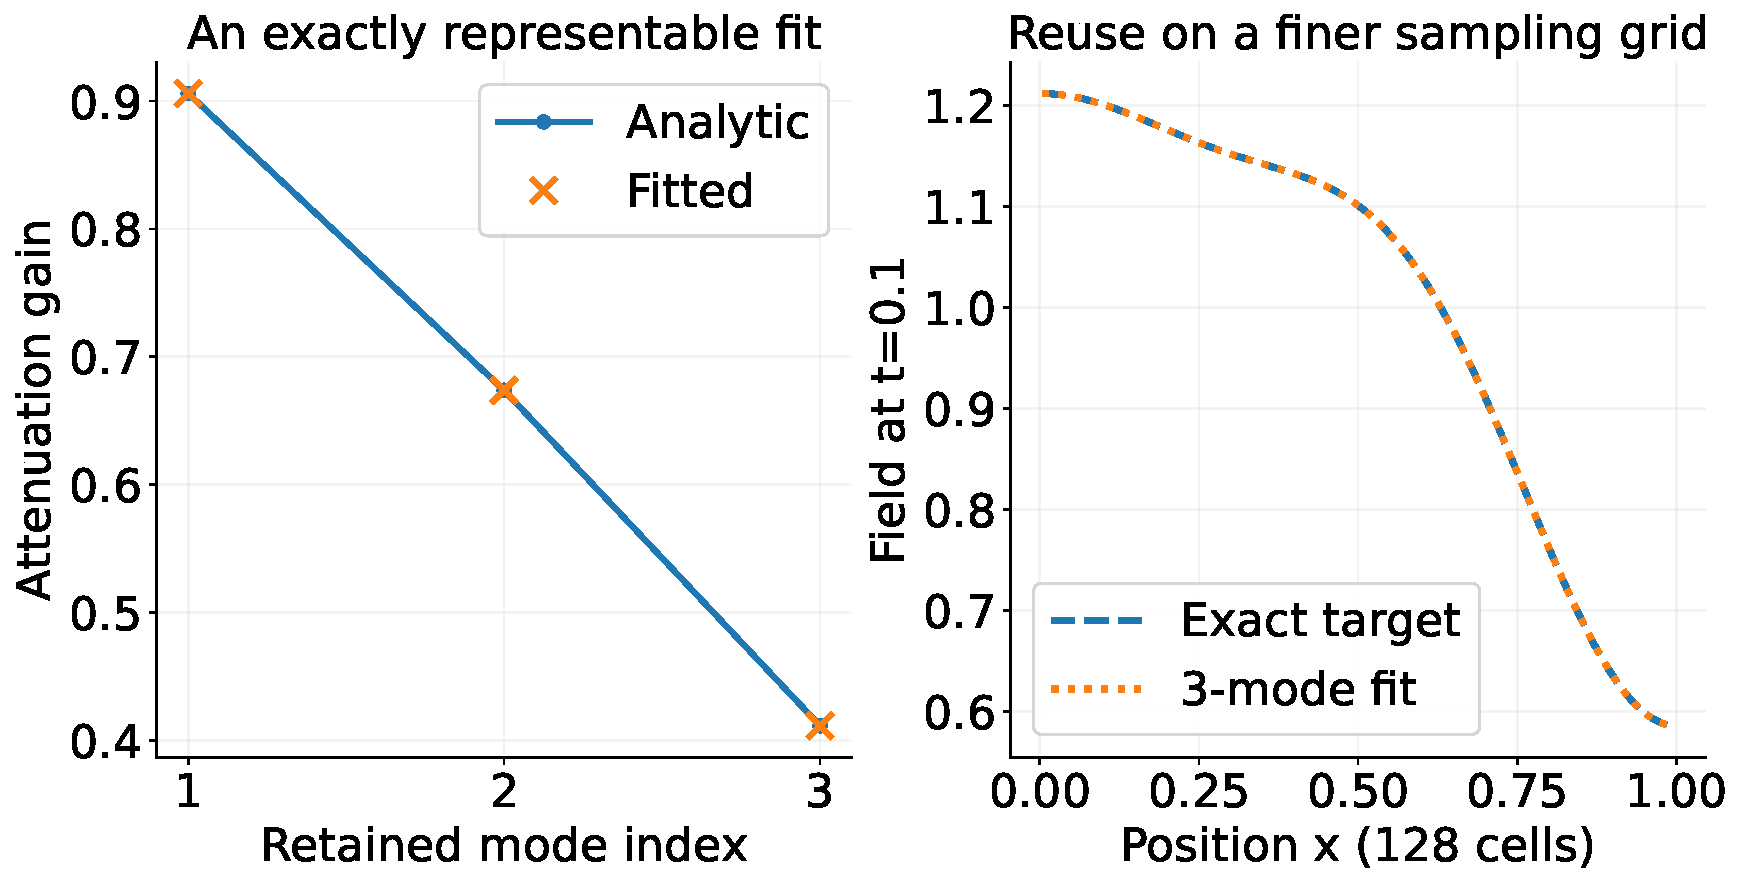
\includegraphics[width=.96\linewidth,height=.57\textheight,keepaspectratio]{spectral-baseline.pdf}\par\smallskip
{\small Original least-squares gains for three heat modes and reuse on a finer grid. Near-roundoff error is expected for this matched finite linear family. This is not GFuNK.}
\end{minipage}\end{center}
\Needspace{10\baselineskip}
\section{Resolved-grid reuse and omitted input modes}
\hypertarget{note-resolved-grid-reuse-and-omitted-input-modes}{}\label{note:resolved-grid-reuse-and-omitted-input-modes}
{\small \href{slides.html\#frame=reuse-on-another-resolved-grid\&step=1}{Slides for this section}}\par
The model is fitted on sixty-four midpoint samples and then evaluated on thirty-two, one hundred twenty-eight and two hundred fifty-six samples. On each grid, the input is a new sampling of the same continuous three-mode field. The projection formulas recover the same coefficients and the reconstruction uses the same fitted gains. Errors remain near roundoff because every grid resolves the retained modes and the hypothesis family matches the exact map.

This is a precise but limited form of grid reuse. It does not demonstrate adaptation to a new domain, a different boundary condition or a changed PDE parameter. It also does not recover arbitrarily high frequencies from sparse samples. If the input contains a fourth cosine mode, the three-mode projection drops that component. The output then lacks the corresponding attenuated fourth mode even though its mean remains correct.

A second failure keeps the input bandwidth fixed but changes diffusivity from 0.1 to 0.02. The unchanged gains apply too much smoothing because they were fitted to the original diffusivity. Both failures are deliberate out-of-contract tests. The code reports them separately from same-family grid reuse. A broad label such as generalization would hide which property actually succeeded and which assumptions changed.

A missing fourth mode of amplitude $a_4$ contributes exact output
\[
 a_4e^{-\kappa(4\pi/L)^2T}\cos(4\pi x/L).
\]
A surrogate that discards it has continuous RMS error $|a_4|e^{-\kappa(4\pi/L)^2T}/\sqrt2$ for that isolated mode, while still preserving the mean. Changing $\kappa$ creates another error: the fitted gains remain tied to their original attenuation rates even when the basis is still appropriate.
\begin{center}\begin{minipage}{.98\linewidth}\centering
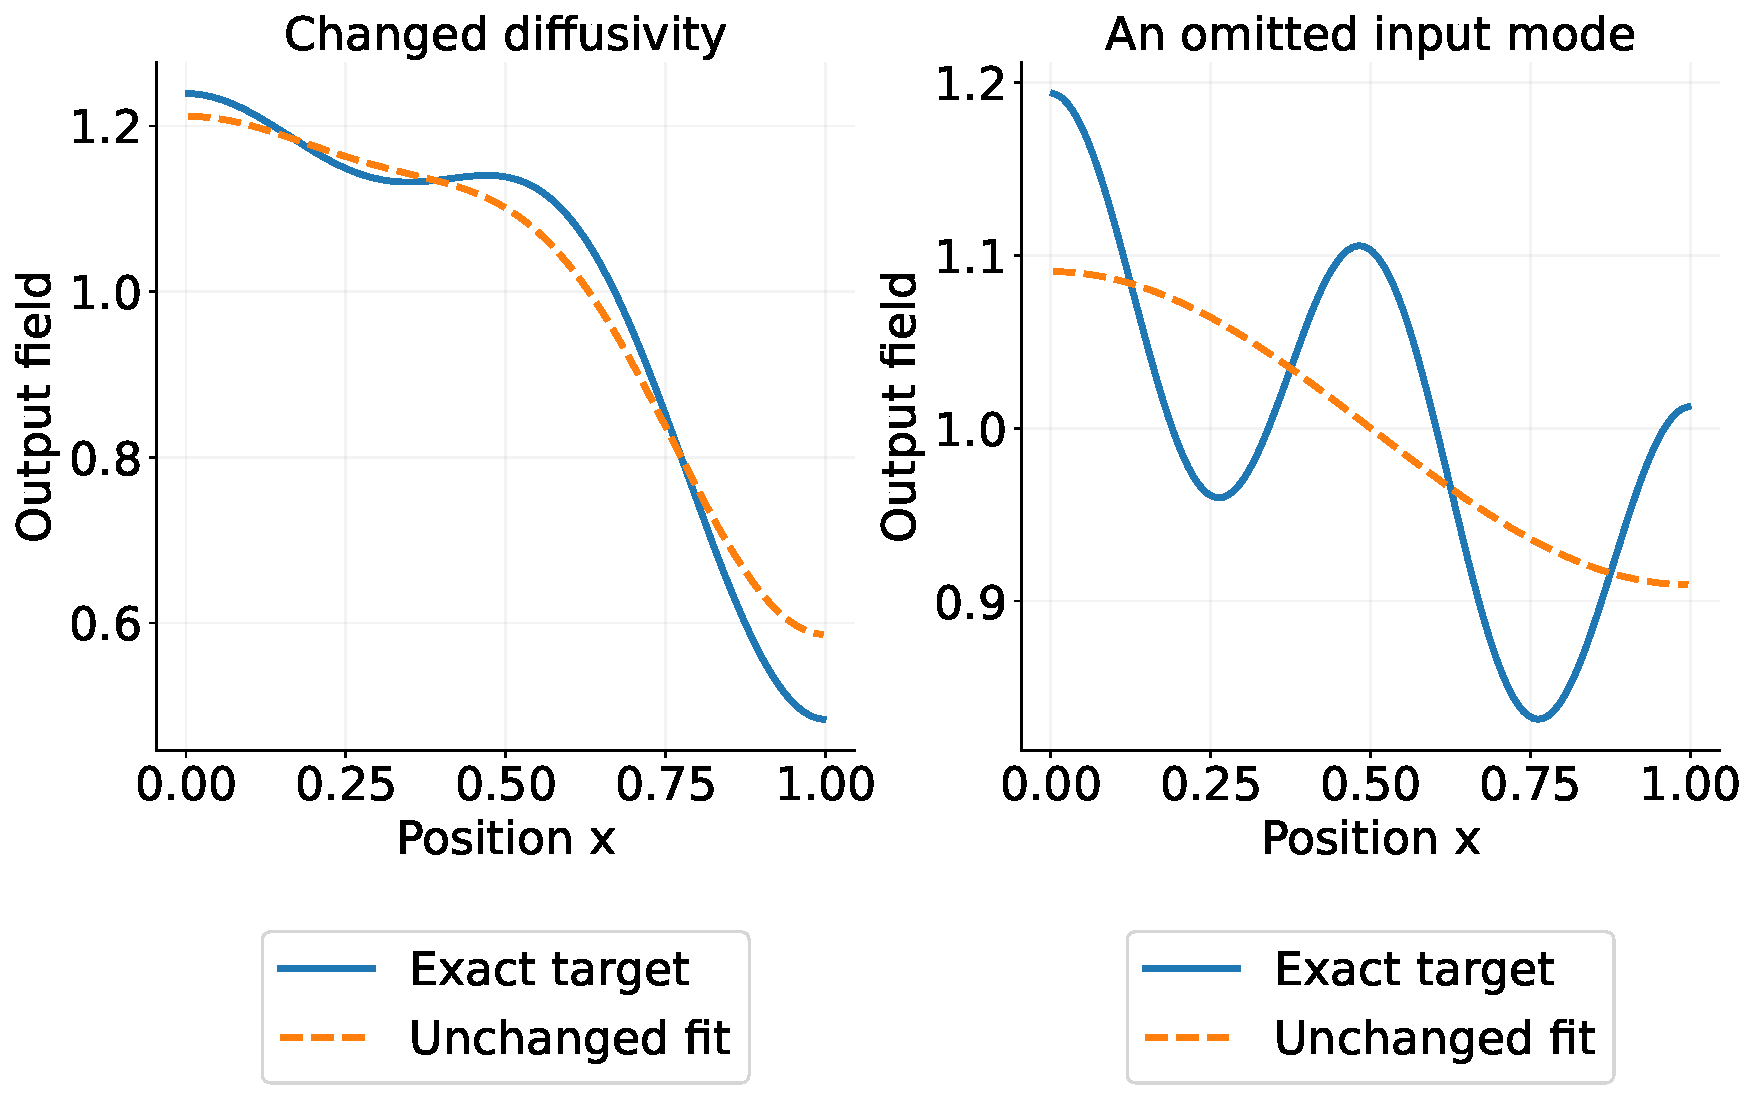
\includegraphics[width=.96\linewidth,height=.57\textheight,keepaspectratio]{transfer-failures.pdf}\par\smallskip
{\small Original changed-diffusivity and omitted-fourth-mode tests. Both preserve the mean while producing field errors; neither is a patient or research-model result.}
\end{minipage}\end{center}
\section{Basis changes and spectral consistency}
\hypertarget{note-basis-changes-and-spectral-consistency}{}\label{note:basis-changes-and-spectral-consistency}
{\small \href{slides.html\#frame=consistent-eigenvector-sign-changes\&step=1}{Slides for this section}}\par
An eigenvector can be multiplied by minus one without changing its eigenvalue. If projection and reconstruction use the same signed basis, the two sign changes cancel in a diagonal spectral map. The companion verifies this algebraic identity for its cosine representation. Comparing raw coefficients across separately constructed bases without their sign conventions, however, can be misleading.

Repeated or nearby eigenvalues create a broader issue: a basis within a degenerate subspace can rotate, and mode ordering can change across related graphs. The GFuNK paper identifies spectral-basis variability and graph-construction choices as limitations. A sign-flip check alone does not settle those questions. Nor does a coordinate rotation test establish robustness to changed geometry or anisotropic parameters. The mathematical transformation and the scientific perturbation must be specified separately.

The paper also reports sensitivity to the inference time step and integration scheme. Learning a generator through a particular discretized rollout can couple the fitted model to that discretization. Switching to a smaller step or higher-order integrator need not improve agreement with the target. Scalar exponential decay provides an example in which this mechanism can be calculated exactly. Our fixed-time three-gain baseline has no learned time generator, so it should not inherit the paper's temporal claims.

Write a diagonal spectral map as $K=\Phi Q\Phi^{\mathsf T}$. For a sign matrix $S$ with entries $\pm1$, replacing $\Phi$ by $\Phi S$ gives the same map because $SQS=Q$. In a repeated-eigenvalue block, a general orthogonal basis change $O$ instead gives $OQO^{\mathsf T}$. It is unchanged for every such $O$ only when the gains are constant on that block. A sign test therefore addresses less than arbitrary eigenspace variability.
\section{Fixed-time maps and learned generators}
\hypertarget{note-fixed-time-maps-and-learned-generators}{}\label{note:fixed-time-maps-and-learned-generators}
{\small \href{slides.html\#frame=the-research-scope-remains-broader\&step=1}{Slides for this section}}\par


The fixed-time gain $q_k$ is not itself a generator coefficient. For exact heat data it equals $e^{-\lambda_kT}$. Recovering a continuous generator would require additional assumptions about positive gains, time dependence and the intended dynamics; the companion performs no such recovery. The subsequent scalar example shows why fitting a generator through a chosen time discretization can introduce a distinct bias.
\bigskip
\section*{Exercises}
\par\noindent\begin{minipage}{\linewidth}
\subsection*{E1. Fit and identify one gain}
Training coefficients are a=\allowbreak{}[1,2,-1] and b=\allowbreak{}[0.8,1.6,-0.8].

\textbf{a} Compute the least-squares gain and residual sum of squares.

\end{minipage}\par\medskip
\textbf{b} What if all three input coefficients were zero?

\par\noindent\begin{minipage}{\linewidth}
\subsection*{E2. A correct mean with a wrong field}
The exact target is 1+\allowbreak{}0.1 cos(4$\pi$x) on[0,1], while a truncated predictor returns 1.

\textbf{a} Compute the mean error and continuous RMS field error.

\end{minipage}\par\medskip
\textbf{b} Compute relative L$^2$ error and interpret the result.

\par\noindent\begin{minipage}{\linewidth}
\subsection*{E3. A normalized graph null mode}
Let W be symmetric nonnegative adjacency with positive degrees Dii=\allowbreak{}sum\_j Wij.

\textbf{a} Show that L\_sym sqrt(D)1=\allowbreak{}0 for L\_sym=\allowbreak{}I-D\textasciicircum{}(-1/2) W D\textasciicircum{}(-1/2).

\end{minipage}\par\medskip
\textbf{b} May you conclude that an arbitrary normalized-graph evolution conserves an unweighted physical mean?

\par\noindent\begin{minipage}{\linewidth}
\subsection*{E4. Separate a baseline from a reproduction}
A report calls the three-gain fit a reproduction of GFuNK because it uses spectral coefficients.

\textbf{a} Rewrite the claim accurately.

\end{minipage}\par\medskip
\textbf{b} Name two additional tests before claiming transfer beyond the fitted family.

\section*{References}
\noindent\begin{minipage}{\linewidth}
Zan Ahmad, Advanced Topics in Computational Cardiology syllabus, Fall 2024. PDF pages 1--2.

\end{minipage}\par\medskip
\noindent\begin{minipage}{\linewidth}
Loeffler, Ahmad, Chen and collaborators, Graph Fourier Neural Kernels: Learning Full PDE Trajectories Across Geometries and Anisotropic Parameter Fields. Main text pages 3,12--18; SI sectionS 7, SI 13--14 / PDF 34--35.

\end{minipage}\par\medskip
\end{document}
